\section{La experiencia: los portafolios reflexivos digitales}\label{sec-laexperiencialos.tex}
	
La experiencia fue realizada durante el primer semestre académico de los
años 2022 y 2023, en la asignatura de Proyectos Didácticos y Evaluativos
Innovadores de la carrera de Pedagogía en Educación Media
Científico-Humanista con mención en Lenguaje de una universidad pública.
Cabe precisar que dicha asignatura es uno de los últimos cursos para
obtener el grado de profesor y, por lo mismo, está ligada al desarrollo
de la práctica profesional, la cual se realiza en el nivel de secundaria
en las aulas chilenas. La mayoría de quienes ingresan a dicha carrera
tienen un rango de edad de 23 a 28 años, aproximadamente.

Se propuso, a los futuros docentes, que los portafolios fueran
construidos a través de etapas y que estos reflejaran su proceso de
práctica profesional en la especialidad. Para ello, se acordaron
sesiones de trabajo en conjunto, donde los futuros docentes podían, a
través del diálogo, dar cuenta del progreso de sus portafolios, sus
principales dificultades y recibir retroalimentación de sus compañeros.
En dichas sesiones, se pudo dialogar sobre las experiencias de mediación
de la literatura realizadas, en las que se discutió sobre las
principales dificultades para llevarlas a cabo.

El formato de portafolio digital fue escogido por su ``potencial de
interactividad y por la posibilidad de construir un texto multimodal e
hipertextual que pueda compartirse en la red por parte de la comunidad''
\cite[p. 15]{gonzalezmontmany2019} y, de este modo, los futuros docentes
pudiesen desplegar sus literacidades digitales a través de la
elaboración de diferentes itinerarios, que reflejaran su autonomía y
creatividad en el proceso de reflexionar en torno a su experiencia de
práctica profesional.

El portafolio digital, además, permite que el futuro docente pueda ver
la progresión de su proceso de aprendizaje, reflexionar en un entorno de
naturaleza dinámica, desarrollar competencias transversales y la
digital, además de crear un ambiente de aprendizaje autónomo en el cual
desarrollar su creatividad \cite{pujola_suarez_2019}.

Se propuso la realización de los portafolios en la plataforma Sites de
Google, ya que los estudiantes de pedagogía poseen una cuenta
institucional que facilita su ingreso y uso de la plataforma y, también,
por el tipo de interfaz que posee, la cual es intuitiva y, por lo tanto,
fácil para incrustar vídeos, imágenes y otros soportes.~

La estructura del portafolio se hizo siguiendo los lineamientos de
\textcite{gonzalez_pujola_2008} tomando como referencia cuatro momentos:
introducción, punto de partida, repertorio de muestras y visión global.
Para el desarrollo de dichos aspectos se realizó una consulta abierta a
través de formularios de Google, cuyo objetivo era democratizar e
individualizar el proceso de creación del portafolio para que los
futuros docentes pudieran desarrollar sus prácticas de literacidad
digital. En los anexos se puede acceder a la secuencia considerada para
la realización del portafolio.

Los portafolios que se presentan en la \Cref{tab-01} fueron seleccionados de
un universo de 14 portafolios digitales. Es necesario señalar que las y
los autores de dichos portafolios, fueron contactados vía correo
electrónico y solicitada su autorización para divulgación, la cual fue
aceptada. Para la selección de los portafolios se consideraron los
Objetivos de Aprendizaje (OA, en \cref{sec-annex} ) trabajados en las prácticas
profesionales, los cuales debían incluir habilidades vinculadas a la
lectura y valoración de textos literarios y, por lo tanto, que
permitieran experiencias de mediación de la literatura en la narración
de la experiencia. Cabe precisar que los OA están de acuerdo con las
Bases curriculares del Ministerio de Educación de Chile (MINEDUC) y
contienen los conocimientos, habilidades y actitudes necesarias para
lograr el aprendizaje. Los OA tienen un orden progresivo y se
desarrollan en los diferentes niveles de educación en Chile, divididos
en básica (1º a 6º básico) y media (7º a 4º medio).

Otro de los criterios de selección fue la utilización de tecnologías
digitales, que atendieran a las características sugeridas por \textcite{costa2019multimodalidad} para la elaboración de portafolios que son la
multimodalidad (estructura formal y recursos semióticos), la
hipertextualidad (creación de itinerarios libres) y la creatividad
(acción singular). En este sentido, los portafolios que fueron
excluidos, además de atender parcialmente a los criterios señalados, no
centraron su secuencia didáctica en OA de literatura o de análisis
literario, sino parcialmente.

Por último, se consideró la diversidad de los centros educativos de la
práctica profesional que pudiera dar cuenta de realidades diferentes.
Especialmente, escuelas con alto índice de vulnerabilidad y que cuyas
características (educación privada o particular, pública, subvencionada
o administración delegada), pudieran influir en el tipo de mediación
realizada. Cabe precisar que, luego de la situación de emergencia
sanitaria, los futuros docentes tuvieron que enfrentar una escuela con
episodios de violencia y estudiantes desescolarizados \cite{figueroa2022escuela} (\Cref{tab-01}).
	
\begin{table}[!htpb]
\centering
\begin{threeparttable}
\caption{Descripción de portafolios digitales seleccionados.}
\label{tab-01}
\begin{tabular}{lp{2cm}ll}
\toprule
Nombre portafolio & OA/unidad trabajada & Nivel & Tipo de escuela\\
\midrule
\href{https://sites.google.com/view/portafolio-sergio-gonzlez/practicando-ando}{Practicando-Ando} & OA8/El amor y la lírica & 8º básico & Particular \\
\href{https://sites.google.com/view/portafolio-pdye/inicio}{Portafolio Pdye} & OA2 & 3º medio & Pública \\
\href{https://sites.google.com/view/portafoliojos/inicio}{Portafolio J} & OA1 & 3º medio & Particular \\
\href{https://sites.google.com/view/portafolio-nicolas-lagos/inicio}{Portafolio NL} & OA4 & 2º medio & Subvencionada \\
\href{https://sites.google.com/view/rosaerium-portaflores/inicio}{Portaflores} & OA2 & 2º medio & Pública/Bicentenario \\
\href{https://sites.google.com/ug.uchile.cl/sacarlavoz/inicio}{Sacar la voz} & OA3/Literatura de terror y ciencia ficción & 8º básico & Pública/Bicentenario \\
\bottomrule
\end{tabular}
\source{Elaboración propia.}
\end{threeparttable}
\end{table}
	
\subsection{Valoración de los portafolios desde las literacidades digitales y pedagogía de las multiliteracidades para la mediación lectora}\label{sub-sec-valorazióndelos}

La valoración de los portafolios y de las experiencias de mediación introducidas en ellos, se realizó a través de dos enfoques principalmente. El primero de ellos corresponde a las literacidades digitales desplegadas en los portafolios. Para ello, se realizó una revisión sobre modelos o marcos desarrollados para las literacidades digitales \cite{gillen_barton_2010,hafner_chik_jones_2015} y se seleccionaron aquellas dimensiones que podrían responder al objetivo de la experiencia, como se puede apreciar en la \Cref{tab-02}.
	
\begin{table}[!htpb]
\centering
\begin{threeparttable}
\caption{Dimensiones de las literacidades digitales para la valoración de los portafolios.}
\label{tab-02}
\begin{tabular}{p{3cm} p{4cm} p{5cm} }
\toprule
Dimensión & Definición & Ejemplo \\
\midrule
Desarrollo cognitivo \cite{gillen_barton_2010} & Vinculación con el pensamiento crítico o la práctica cultural y crítica. & Ideología sobre la mediación lectora/visión de la literatura/ visión de las prácticas de literacidad. \\
Significado \cite{hafner_chik_jones_2015} & Formas de representación y uso de herramientas de creación multidisciplinarias & Uso de hipertexto/multi\-mo\-da\-li\-dad/ selección de herramientas digitales para relatar la experiencia/ uso de redes sociales y participación en la cultura. \\
Autenticidad y acceso \cite{gillen_barton_2010} & Inclusión digital y de la ciudadanía digital. Identidad digital. & Relación con las herramientas y plataformas/visión docente o mediadora/ presentación de sí mismo en la plataforma digital. \\
\bottomrule
\end{tabular}
\source{Elaboración propia.}
\end{threeparttable}
\end{table}
	
El segundo enfoque corresponde a la visualización de la mediación de la
lectura literaria relatada en los portafolios. Para ello, se atendió a
las estrategias de interpretación desarrolladas, prácticas de
literacidad, visión del estudiante como potencial lector, por medio del
enfoque de la pedagogía de las multiliteracidades \cite{kalantzis2019,Kalantzis2023}.

La pedagogía de las multiliteracidades es un enfoque que considera los
procesos de conocimiento que realizan los estudiantes para aprender y
que incluyen las prácticas de literacidad y literacidades digitales de
quienes participan dentro del aula. Los procesos de conocimiento desde
este enfoque son experimentar lo conocido/lo nuevo; conceptualizar desde
la teoría/ la denominación; analizar crítica o funcionalmente; aplicar
creativamente o de forma apropiada (\Cref{fig-01}).

\begin{figure}[htpb]
\centering
\begin{minipage}{\textwidth}
\caption{procesos de conocimiento de la pedagogía de las multiliteracidades.}
\label{fig-01}
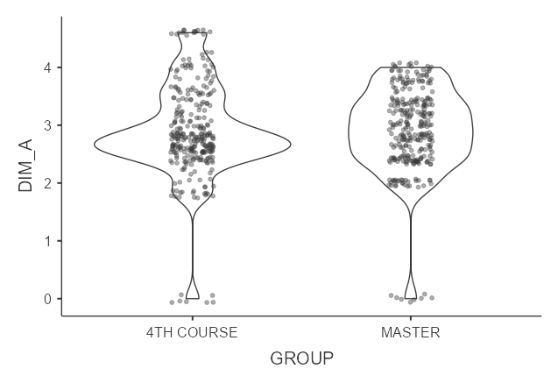
\includegraphics[width=\textwidth]{fig1.png}
\source{Captura de pantalla del libro de \textcite[p. 96]{kalantzis2019} \emph{Las alfabetizaciones múltiples, teoría y práctica}.}
\end{minipage}
\end{figure}
	
Este enfoque fue presentado en sesiones teóricas a los futuros docentes
y discutido dentro de las clases programadas en la asignatura para su
posible inclusión en los proyectos de innovación que serían realizados
en su práctica profesional. Además, se motivó el diseño de experiencias
de mediación de la literatura que incluyeran las prácticas de
literacidad y literacidad digital de sus estudiantes.

A partir de la consideración de ambos enfoques, se elaboraron unos
criterios (\Cref{tab-03}) que, finalmente, apoyaron la valoración de la
experiencia y del despliegue de las literacidades digitales de un grupo
de futuros profesores de lengua y literatura en sus portafolios.

\begin{table}[!htpb]
\centering
\begin{threeparttable}
\caption{Descripción de los criterios utilizados en la valoración de los portafolios.}
\label{tab-03}
\begin{tabular}{lp{5cm}p{5cm}}
\toprule
	& Literacidades digitales & Mediación desde las multiliteracidades. \\
\midrule
Desarrollo cognitivo & Despliegue de literacidades digitales desde la visión de la cultura de la web/ motivación del uso. & Análisis y/o interpretación. Tipo de lecturas escogidas. Encuadre: experimentar desde lo conocido o lo nuevo. \\
Significado & Uso de la plataforma Sites. Multimodalidad. Hipertextualidad/uso de enlaces. & Agencia del estudiantado (herramientas de creación). Aplicar creativamente y/o apropiadamente. \\
Autenticidad y acceso & Selección de herramientas y tipo de uso. Presentación desde la identidad digital. & Mediación a partir de alguno de los procesos de conocimiento de las multiliteracidades. \\
\bottomrule	
\end{tabular}
\source{Elaboración propia.}
\end{threeparttable}
\end{table}

\subsection{Valoración de las literacidades digitales y mediación de la literatura}\label{sub-sec-valoracióndelas}
	A continuación, se expondrá la valoración de los portafolios desde las
	dimensiones de las literacidades digitales y el enfoque de la pedagogía
	de las multiliteracidades, por medio de los criterios expuestos en el
	apartado anterior.

\subsubsection{Desarrollo cognitivo}\label{sub-sub-sub-sec-desarrollo}

Esta dimensión se valoró desde la visión de la cultura de internet y las
redes sociales. La mediación desde las multiliteracidades se apreció
desde el encuadre y el tipo de análisis propuesto.

Desde la perspectiva de las literacidades digitales, se pudo observar en
algunos portafolios el uso de memes y el lenguaje de las redes sociales
(\Cref{fig-02}). Sin embargo, dicho uso no fue común en la totalidad de los
portafolios valorados, ya que en varios de ellos se observó la presencia
de prácticas de literacidad que pertenecen al ámbito académico, cuyo
énfasis está en el código escrito. No obstante, dicho código estaba
acompañado de vídeos, audios e imágenes.

\begin{figure}[htpb]
\centering
\begin{minipage}{.7\textwidth}
\caption{Uso de memes vinculados con la cultura de internet y que fueron utilizados en la reflexión realizada por el docente en formación en su portafolio.}
\label{fig-02}
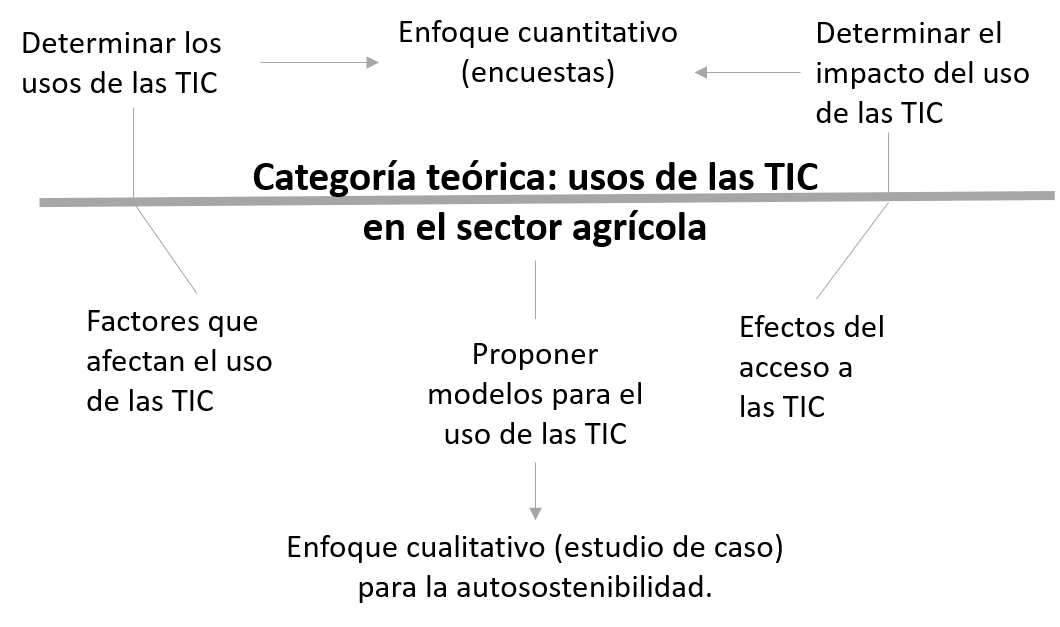
\includegraphics[width=\textwidth]{fig2.png}
\source{Captura de pantalla del portafolio ``\href{https://sites.google.com/view/portafolio-sergio-gonzlez}{Practicando -ando}''.}
\end{minipage}
\end{figure}

En algunos portafolios se puede visualizar que los futuros profesores
utilizaron la gamificación para explicar sus trayectorias o para
introducir al lector en un ámbito reflexivo nuevo. Esto fue uno de los
aspectos que sobresalió dentro de los portafolios visualizados. Sin
embargo, en rasgos generales, se puede señalar que prefieren utilizar la
interfaz proporcionada por Sites por defecto, sin alterarla demasiado.

Dentro de esta dimensión, lo que refiere a las experiencias de mediación
relatadas, en la mayoría de los portafolios se pudo observar que se
realizaban desde el proceso de conocimiento de experimentar lo nuevo, ya
que eran los profesores en formación quienes presentaban un recurso que
pudiera ser del interés de sus estudiantes y que, luego de su análisis y
discusión, era utilizado para presentar el texto literario que sería
interpretado, como se puede apreciar en la \Cref{tab-04}.

\begin{table}[!htpb]
\centering
\begin{threeparttable}
\caption{Ejemplo de recursos utilizados dentro del proceso ``experimentar lo nuevo'' conectado con el análisis e interpretación de obras literarias.}
\label{tab-04}
\begin{tabular}{llp{3cm}p{3cm}p{3cm}}
\toprule
Portafolio & OA & Recurso & Proceso de conocimiento & Obra literaria \\
\midrule
Practicando-ando & OA8 & Vídeo
\href{https://youtu.be/DUGtyj5QlEM?si=_KwsI8ND0PrJCqJ3}{``Dos oruguitas}'' (Sebastián Yatra). & Experimentar lo nuevo. Conceptualizar desde la teoría. & Poema de Emily Dickinson. \\
Portafolio NL & OA4 & \href{https://sites.google.com/view/portafolio-nicolas-lagos/repertorio-de-muestras/segunda-muestra-desafíos}{Canción ``The book of you and I}'' (Alec Benjamin). & Experimentar lo nuevo. Analizar funcional y críticamente. & ``La esperanza es esa cosa con plumas'' Emily Dickinson; ``Espejo'' Silvia Plath. \\
Portaflores & OA2 & Corto animado: ``\href{https://youtu.be/to8yh83jlXg?si=rPhsC7o_mtj8rDCp}{The last Bastion}'' (Overwatch). Microcuento \href{https://santiagoen100palabras.cl/en-vitrina/}{``En vitrina''} (Valentina Sandoval). & Experimentar lo conocido/lo nuevo. & Tema del viaje. \\ 
\bottomrule
\end{tabular}
\end{threeparttable}
\end{table}
	
\subsubsection{Significado}\label{sub-sub-sec-significado}

Esta dimensión se valoró a través del uso que realizaron los docentes en
formación de la plataforma Sites, la idea de diseño desde la
multimodalidad y el hipertexto desde la creación de itinerarios libres.
A su vez, se procuró observar el desarrollo de la agencia del
estudiantado a través del proceso de conocimiento de aplicar de forma
apropiada o creativa, u otro vinculado a las multiliteracidades, en las
experiencias de mediación presentadas según el OA escogido.

Se puede señalar que, en forma general, en los portafolios observados se
utiliza el hipertexto como una forma de expresión y creación dentro de
la plataforma Sites. Una de las plataformas que permitió estos
itinerarios fue Genially, ya que en algunos portafolios fue la base de
los itinerarios propuestos (\Cref{fig-03}) plataforma permite una
interacción y navegación entre diversos hipervínculos. Otra herramienta
que permitió la creación de itinerarios, fue Slides de Google, ya que la
misma plataforma Sites facilita su inserción.

\begin{figure}[htpb]
\centering
\begin{minipage}{.7\textwidth}
\caption{ejemplo de un itinerario propuesto a través de la herramienta Genially.}
\label{fig-03}
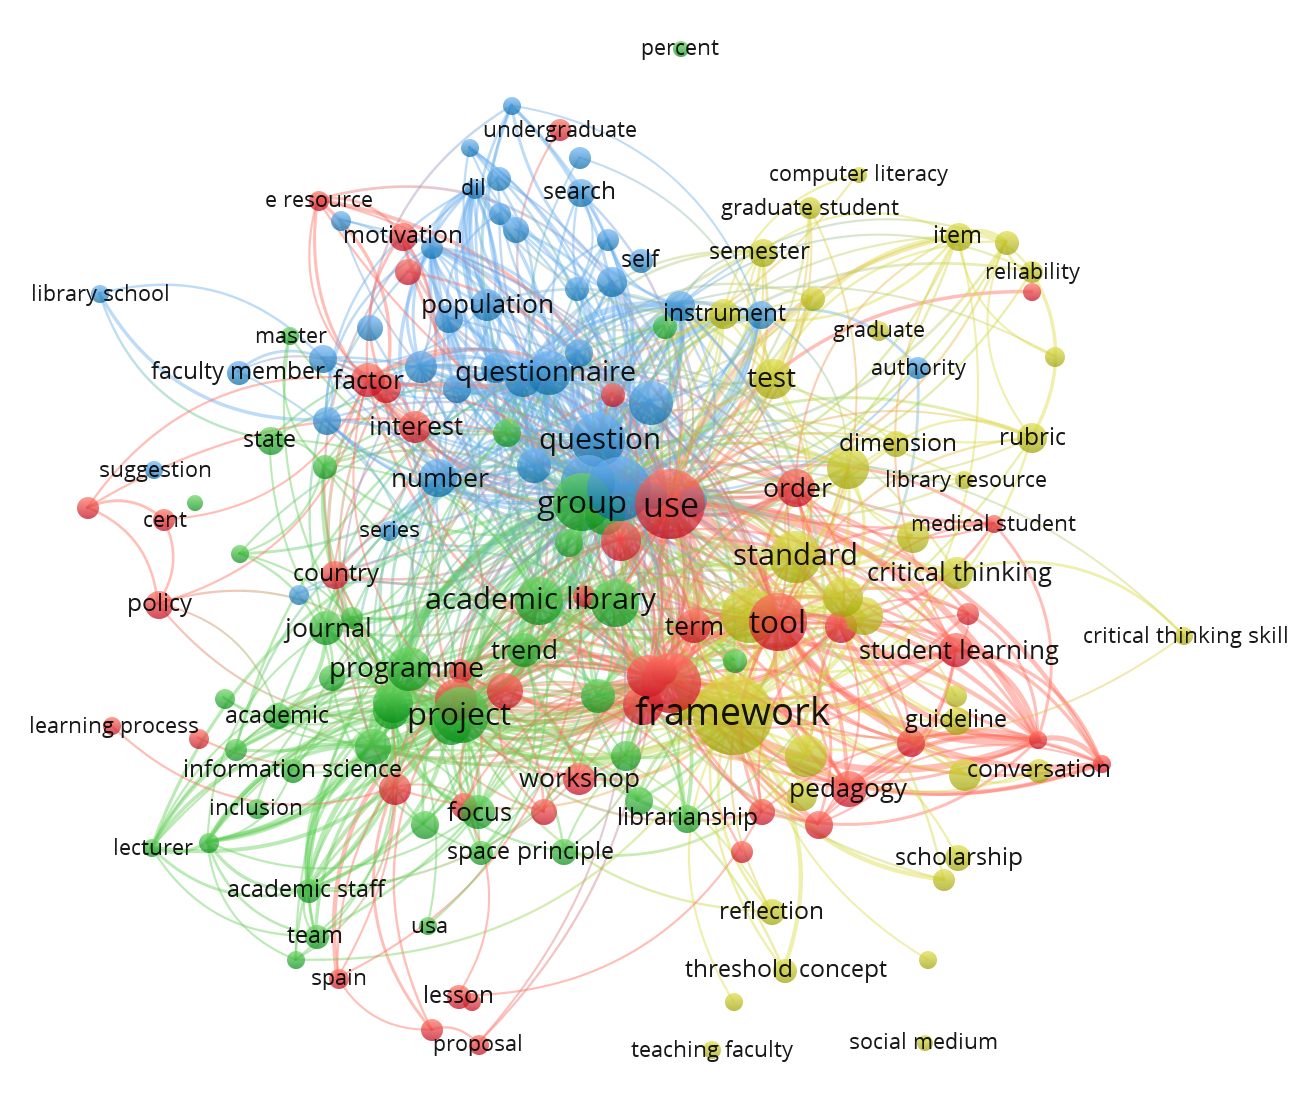
\includegraphics[width=\textwidth]{fig3}
\source{Captura de pantalla del portafolio ``\href{https://sites.google.com/view/rosaerium-portaflores/has-llegado-a-tu-nuevo-destino/misión-2-hay-un-extraño-no-no-soy-yo}{Portaflores}''.}
\end{minipage}
\end{figure}


La combinación de recursos que permite la plataforma Sites, facilitó a
los futuros docentes diseñar su portafolio como un texto multimodal e
hipertextual y, por tanto, que cada uno de los portafolios lograra un
diseño particular y único.

El uso de diferentes recursos dentro de los portafolios digitales se
enlaza de alguna manera con los procesos de mediación de la lectura
presentados. Esto pudo observarse a través de la aplicación apropiada o
creativa según el proceso de conocimiento de las multiliteracidades
escogido. Algunas de las actividades realizadas bajo dicho proceso,
fueron concebidas para que los estudiantes de aula pudieran comprender
los conceptos que les servirían para analizar textos literarios de
acuerdo con el OA de la secuencia planificada (\Cref{fig-04}). Con este fin,
los futuros docentes recurrieron al uso de recursos digitales conocidos
y utilizados en sus portafolios.

\begin{figure}[htpb]
\centering
\begin{minipage}{.7\textwidth}
\caption{Ejemplo de actividad de mediación de acuerdo al OA 4, la creación de un diccionario simbólico a través de la herramienta Padlet.}
\label{fig-04}
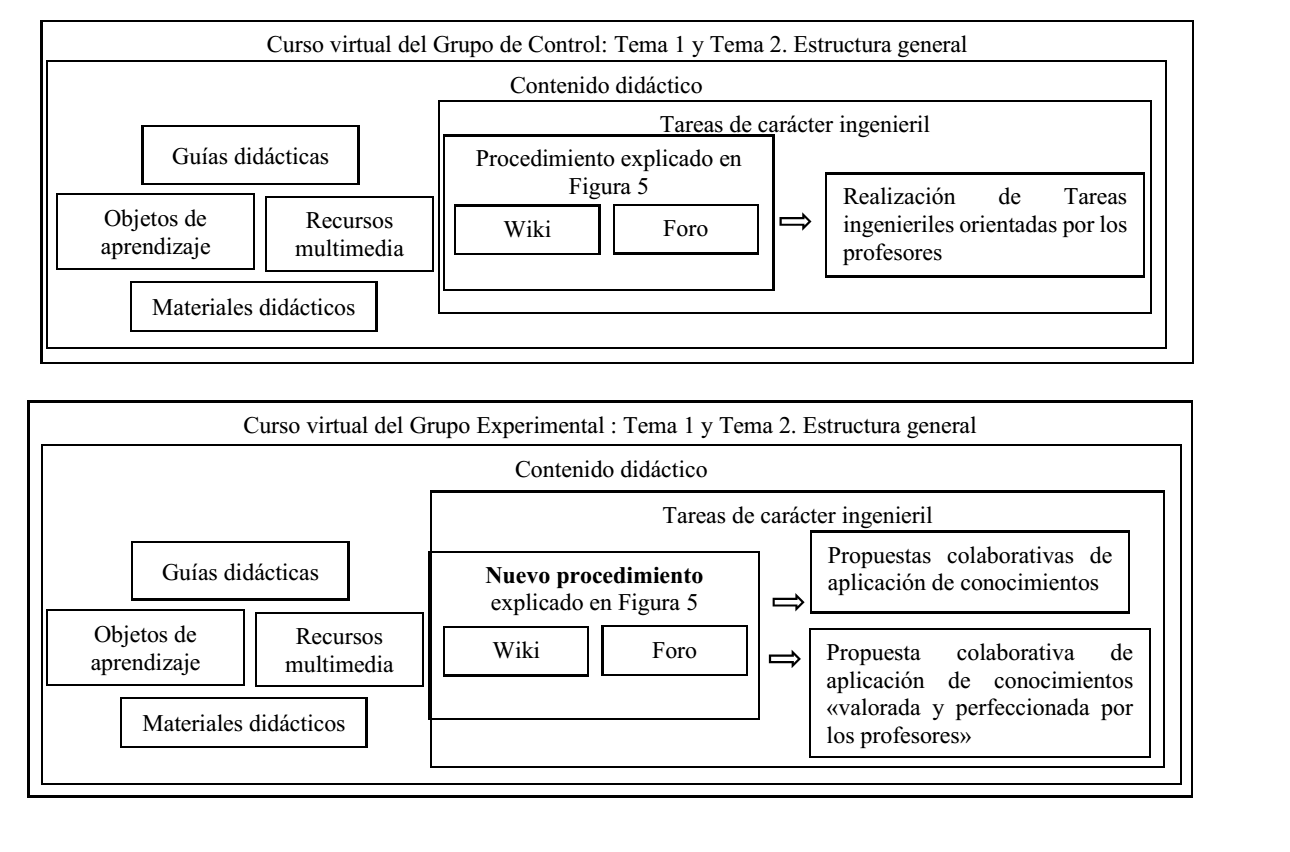
\includegraphics[width=\textwidth]{fig4.png}
\source{Captura de pantalla del portafolio ``\href{https://sites.google.com/view/portafolio-nicolas-lagos/repertorio-de-muestras/segunda-muestra-desafíos}{Portafolio NL}''.}
\end{minipage}
\end{figure}

\subsubsection{Autenticidad y acceso}\label{sub-sub-sec-autenticidad}

En esta dimensión se valoró a los portafolios desde la selección de
herramientas digitales y su uso. Desde la experiencia de mediación,
interesaba observar la proyección de los procesos de conocimiento de las
multiliteracidades narrados en los portafolios.

En todos los portafolios, la herramienta más utilizada fue Genially, ya
que es una plataforma que permite la interactividad y la creación de
textos multimodales. Otras de las herramientas utilizadas fueron Padlet
y YouTube.

Cabe precisar que el diseño de la plataforma Sites fue utilizado por
defecto en el diseño de los portafolios, sobre todo en lo que respecta
al uso de pestañas como hipervínculos. En esto último, también fue muy
utilizada la plataforma Slides y Docs de Google, ya que la plataforma
facilitaba la inserción de estos recursos.

En el caso de YouTube, este fue empleado para exponer vídeos generados
por Zoom, semejante, en este sentido, a una exposición oral. También
dicha plataforma fue utilizada en algunos casos como \emph{podcast}
(\Cref{fig-05}) y, por tanto, sin el énfasis divulgativo y social inherente a
esta plataforma.

\begin{figure}[htpb]
\centering
\begin{minipage}{\textwidth}
\caption{Ejemplo de uso de la plataforma YouTube como \emph{podcast.}}
\label{fig-05}
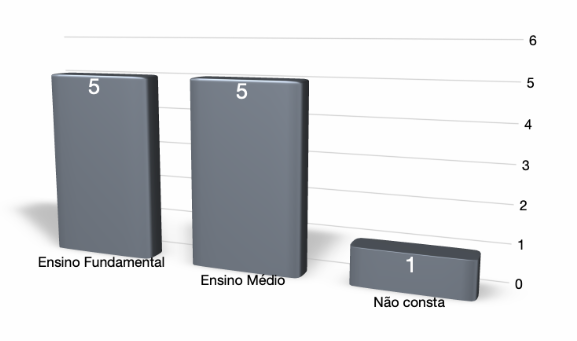
\includegraphics[width=\textwidth]{fig5}
\source{Captura de pantalla del portafolio ``\href{https://sites.google.com/view/portafolio-pdye/introducción}{Portafolio Pdye}''.}
\end{minipage}
\end{figure}

Sobre esto último, es necesario mencionar que, en la valoración de los
portafolios, se pudo distinguir que hay un predominio de prácticas de
literacidad académicas, ya que el código escrito estaba presente en la
mayoría de las presentaciones realizadas (con Slides y Genially) y en el
contenido de las pestañas de los portafolios.

Lo anterior se condice, en cierto modo, con el desarrollo de las
experiencias de mediación, ya que, dentro de los procesos de
conocimiento de las multiliteracidades, hay un predominio de la
experimentación desde lo nuevo, que da paso a estrategias tradicionales
de lectura desarrolladas a través de procesos psico-cognitivos. Los
espacios de discusión y análisis de los textos literarios se dan dentro
de los procesos de experimentación o análisis crítico. Los procesos de
conceptualización son los menos abordados.
